\documentclass{article}
\usepackage{amsmath} %Never write a paper without using amsmath for its many new commands
\usepackage{amssymb} %Some extra symbols
\usepackage{makeidx} %If you want to generate an index, automatically
\usepackage{graphicx} %If you want to include postscript graphics
%%%  \usepackage{mystyle} 
%Create your own file, mystyle.sty where you put all your own \newcommand statements
%%%
%%%
\usepackage{amscd}

\usepackage{Sweave}


%%\VignetteIndexEntry{Example hodograms}

%%% \usepackage{Sweave}

\begin{document}

%%%\renewcommand\floatpagefraction{.9}
%%%\renewcommand\topfraction{.9}
%%%\renewcommand\bottomfraction{.9}
%%%\renewcommand\textfraction{.1}
%%%\setcounter{totalnumber}{50}
%%%\setcounter{topnumber}{50}
%%%\setcounter{bottomnumber}{50}

\setkeys{Gin}{width=0.9\textwidth}



\numberwithin{equation}{section}

%%%   \SweaveOpts{prefix.string=hodo}



\author{Jonathan M. Lees\\
University of North Carolina, Chapel Hill\\
Department of Geological Sciences\\
CB \#3315, Mitchell Hall\\
Chapel Hill, NC  27599-3315\\
email: jonathan.lees@unc.edu\\
ph: (919) 962-0695
}
%%  \address{University of North Carolina, Chapel Hill}
%% \contact{Jonathan M. Lees}
%% \contactaddress{Department of Geological Sciences, CB #3315, Mitchell Hall, Chapel Hill, NC  27599-3315}
%% \contactemail{jonathan.lees@unc.edu}
%% \contactphone{(919) 962-0695}
\title{Seismic Hodograms in R}
\date{March, 2008}

\maketitle


\begin{abstract}
Plot hodograms (particle motion) for 3-component seismic data.
\end{abstract}

\section{Example}

Start out by calling the RSEIS library,

\begin{Schunk}
\begin{Sinput}
> library(RSEIS)
\end{Sinput}
\end{Schunk}

Then load some data and plot.  This data is from the Coso Geothermal field in Coso Califormia.
The data is sampled at 250 sampled/sec and there are numerous stations recorded
on three components.   Some stations are too noise for particle motion analysis.

\begin{Schunk}
\begin{Sinput}
> data(GH)
> PICK.GEN(GH, SHOWONLY = TRUE)
\end{Sinput}
\end{Schunk}

In this case the GH structure holds the 
phase arrival information as well as the station locations and event location.

\begin{Schunk}
\begin{Sinput}
> print(GH$pickfile$STAS$name)
\end{Sinput}
\begin{Soutput}
 [1] "CE1"  "CE4"  "CE3A" "SM5"  "NV6"  "CE2"  "NV1"  "CE7"  "NV10" "CE8" 
[11] "NV4"  "NV5"  "NV2"  "CE1"  "CE4"  "CE3A" "SM5"  "NV6"  "CE2"  "CE6" 
[21] "CE7"  "CE8"  "NV4"  "NV5" 
\end{Soutput}
\end{Schunk}

We will choose one station and do the hodogram analysis there, but 
our analysis could easily be put in a loop to cover all the stations.

\begin{Schunk}
\begin{Sinput}
> thesta = "CE1"
> iwv = which(GH$STNS == thesta & GH$COMPS == "V")
> iwn = which(GH$STNS == thesta & GH$COMPS == "N")
> iwe = which(GH$STNS == thesta & GH$COMPS == "E")
> data = cbind(GH$JSTR[[iwv]], GH$JSTR[[iwn]], GH$JSTR[[iwe]])
\end{Sinput}
\end{Schunk}

Next we get the station back azimuth to the seismic event, 
which has been located previously.  The information on
the location of the seismic event is stored also in the pickfile.


\begin{Schunk}
\begin{Sinput}
> ipphase = which(GH$pickfile$STAS$name == thesta & GH$pickfile$STAS$phase == 
+     "P")
> isphase = which(GH$pickfile$STAS$name == thesta & GH$pickfile$STAS$phase == 
+     "S")
> lat = GH$pickfile$STAS$lat[ipphase]
> lon = GH$pickfile$STAS$lon[ipphase]
> DAZ = distaz(lat, lon, GH$pickfile$LOC$lat, GH$pickfile$LOC$lon)
> rbaz = grotseis(DAZ$baz, flip = FALSE)
\end{Sinput}
\end{Schunk}

To illustrate the approach we start by plotting 
a map view of the stations and the earthquake source,

\begin{Schunk}
\begin{Sinput}
> plot(c(GH$pickfile$STAS$lon, GH$pickfile$LOC$lon), c(GH$pickfile$STAS$lat, 
+     GH$pickfile$LOC$lat), type = "n", xlab = "LON", ylab = "LAT")
> points(GH$pickfile$STAS$lon, GH$pickfile$STAS$lat, pch = 6)
> points(GH$pickfile$LOC$lon, GH$pickfile$LOC$lat, pch = 8)
> text(GH$pickfile$STAS$lon, GH$pickfile$STAS$lat, GH$pickfile$STAS$name, 
+     pos = 3)
\end{Sinput}
\end{Schunk}
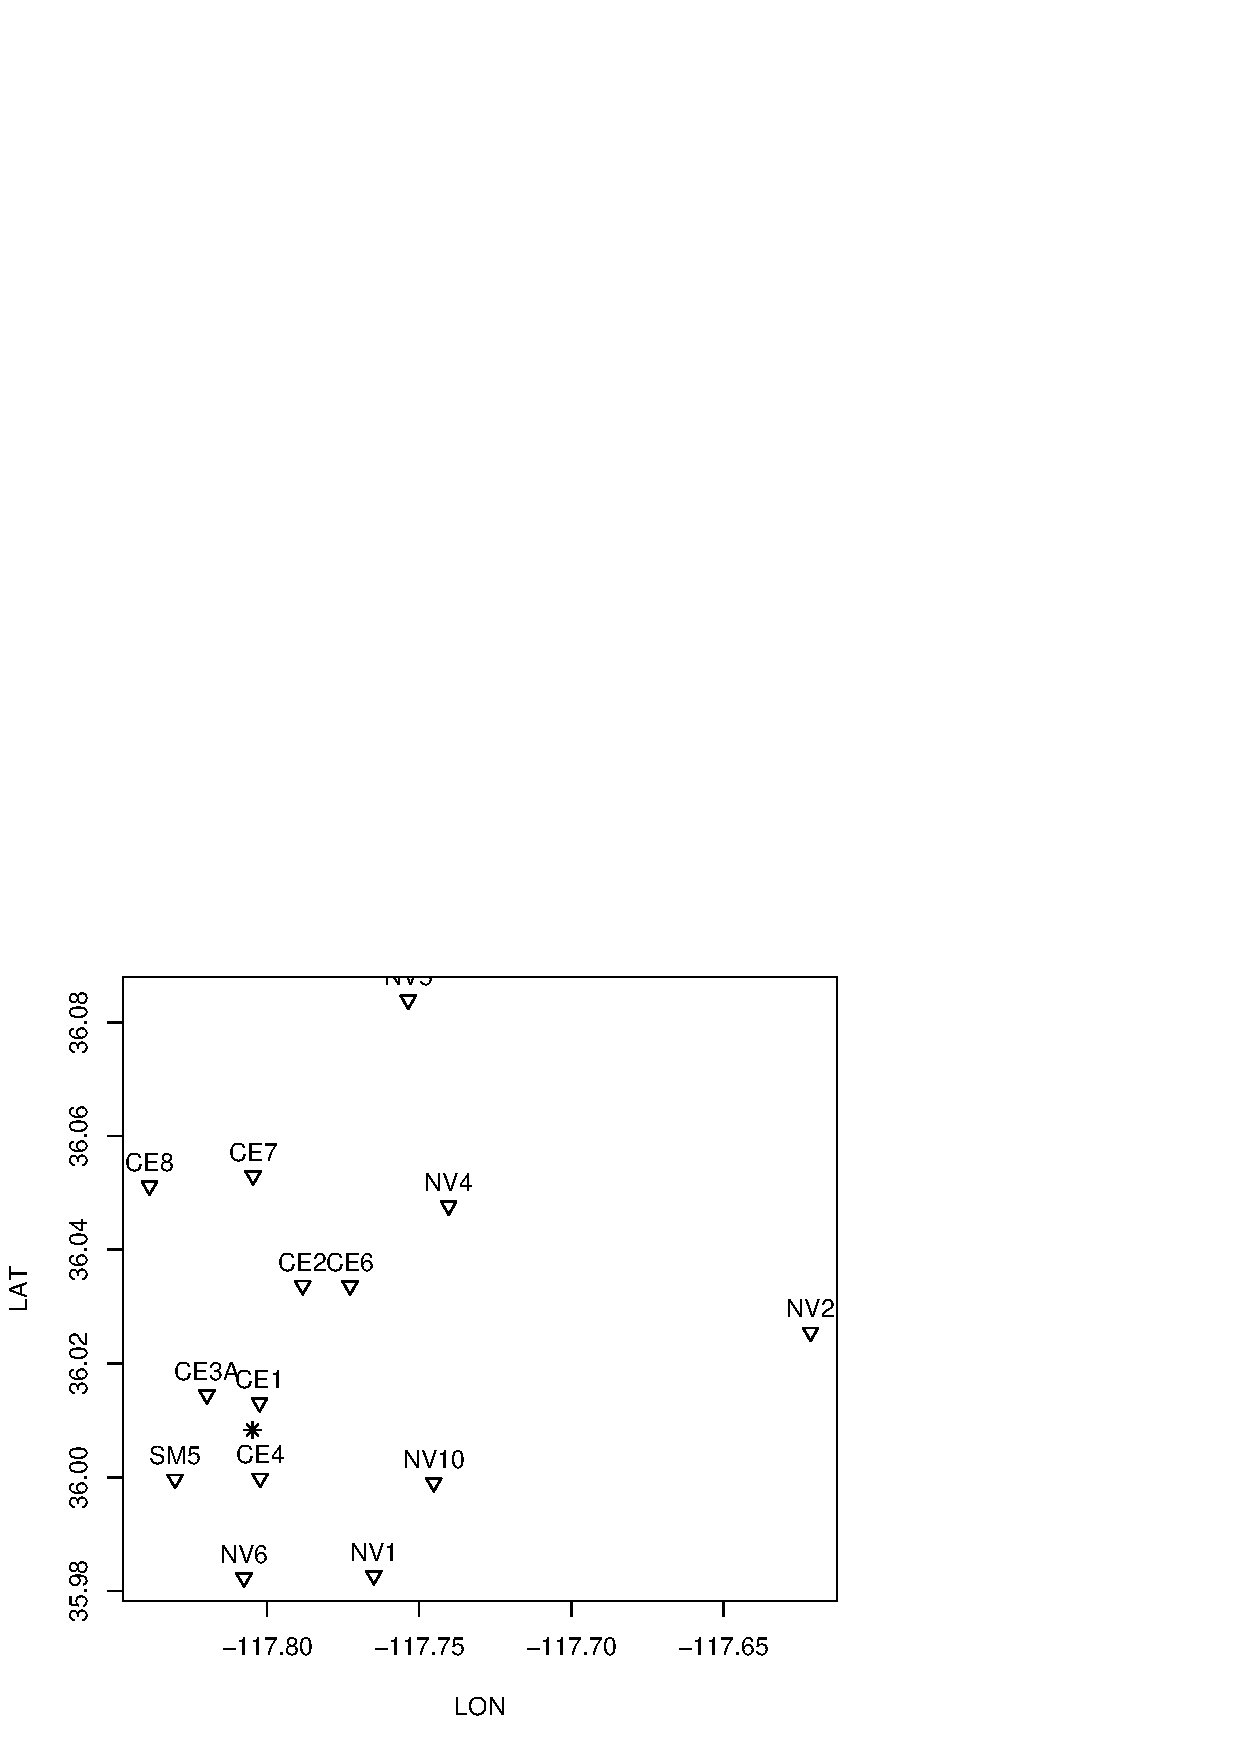
\includegraphics{hodo-006}

These can be plotted in km rather than LAT-LON by either projection
or byu simply using the distances 
to the stations and azimuths to get the approximate flat orientation.
We show the orientation of the horizontal components after the seismogram gets rotated by
the designated angle.  The red arrow is the radial component and the blue
is the transverse.

\begin{Schunk}
\begin{Sinput}
> x = DAZ$dist * sin(DAZ$baz * pi/180)
> y = DAZ$dist * cos(DAZ$baz * pi/180)
> plot(c(0, 1.3 * x), c(0, 1.3 * y), type = "n", asp = 1, xlab = "E-W, km", 
+     ylab = "N-S, km")
> points(c(0, x), c(0, y), pch = c(3, 6))
> text(x, y, labels = "station", pos = 1)
> text(x, y, labels = GH$pickfile$STAS$name[ipphase], pos = 2)
> text(0, 0, labels = "source", pos = 3)
> vecs = rbind(c(0, 0, 1), c(0, 1, 0))
> bvec = vecs %*% rbaz
> bvec = 0.1 * DAZ$dist * bvec
> arrows(x, y, x + bvec[, 2], y + bvec[, 3], col = c("red", "blue"))
\end{Sinput}
\end{Schunk}
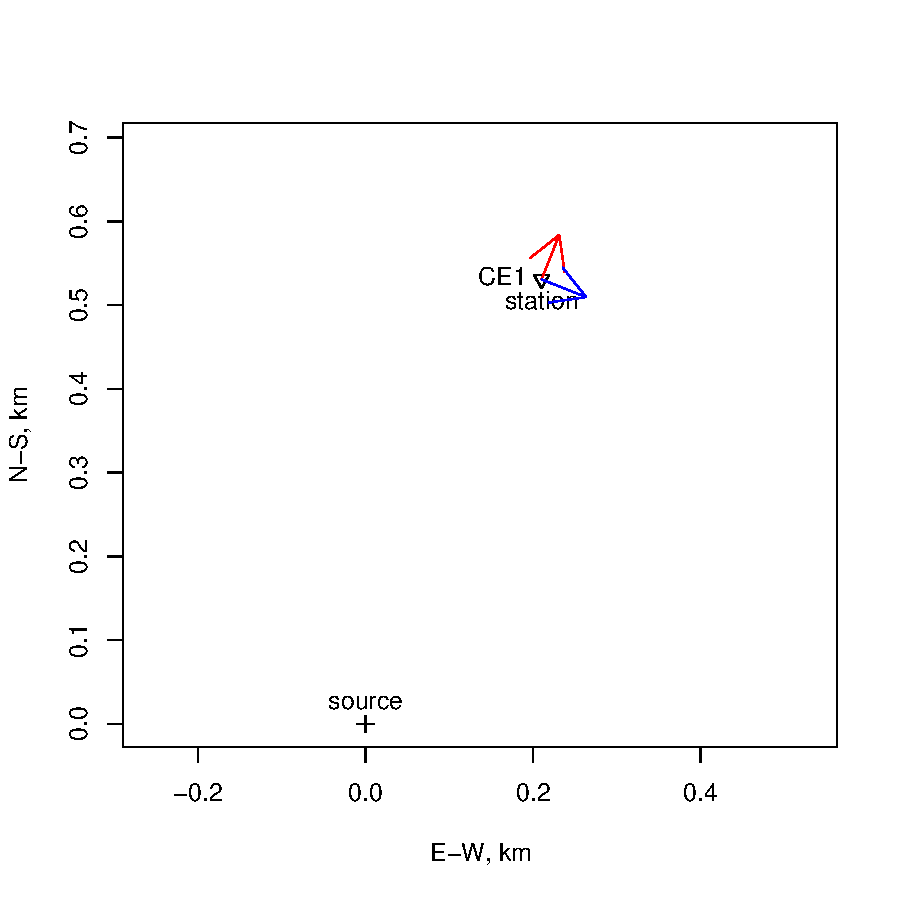
\includegraphics{hodo-007}


We first plot the data in its original Vertical-North-East orientation,

\begin{Schunk}
\begin{Sinput}
> vnelabs = c("Vertical", "North", "East")
> rotlabs = c("Vertical", "Radial(away)", "Transvers(right)")
> xt = seq(from = 0, by = GH$dt[iwv], length = length(GH$JSTR[[iwv]]))
> PLOT.MATN(data, tim = xt, dt = GH$dt[iwv], notes = vnelabs)
\end{Sinput}
\end{Schunk}
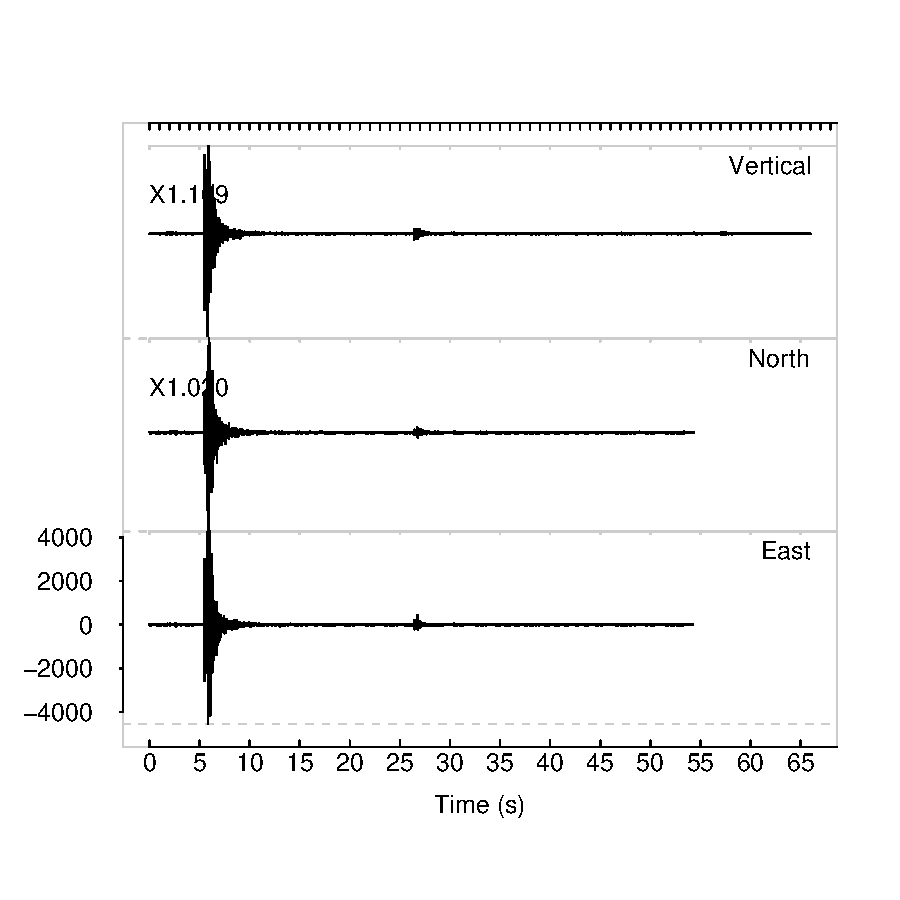
\includegraphics{hodo-008}


And then we rotate the seismograms so that they are oriented 
Vertical-Radial-Transverse, is is often done in seismic analysis:


\begin{Schunk}
\begin{Sinput}
> btemp = data %*% rbaz
> PLOT.MATN(btemp, tim = xt, dt = GH$dt[iwv], notes = rotlabs)
\end{Sinput}
\end{Schunk}
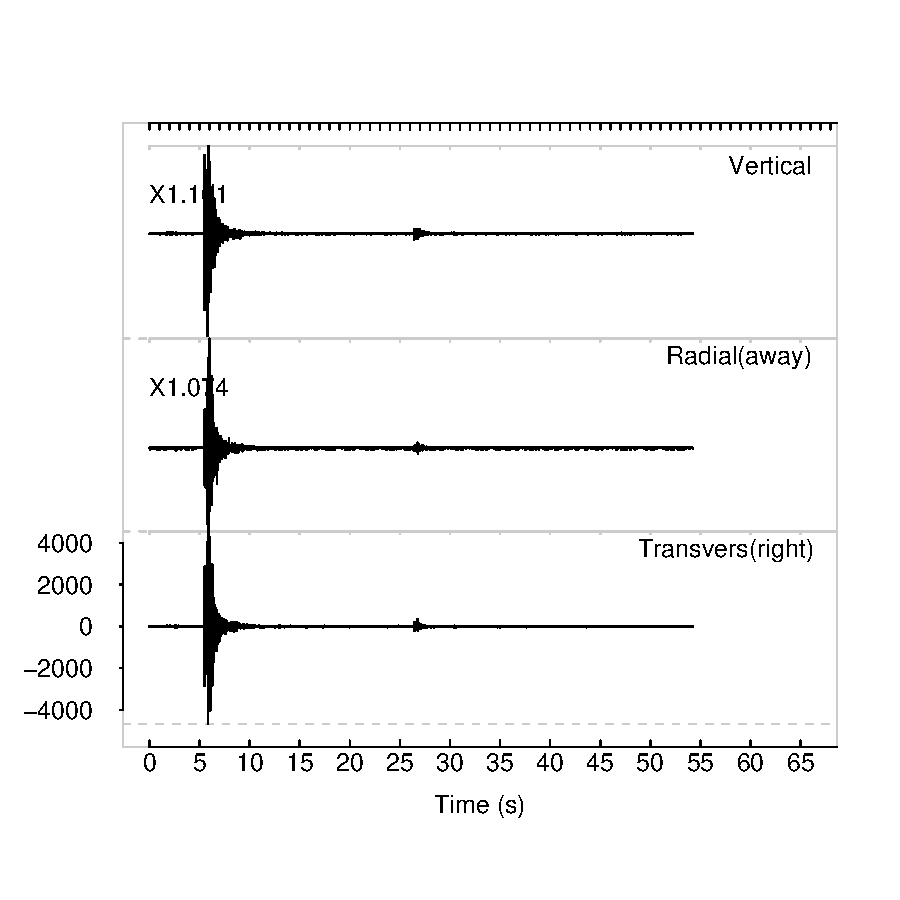
\includegraphics{hodo-009}

Next we extract information from the seismic structure that
tells us when the P and S-arrival were estimated.  This information\
is stored in the pickfile structure,
but we want to know how many seconds paste the start of the trace the
arrivals came in, so we can window that portion of the trace
for hodogram analysis.

\begin{Schunk}
\begin{Sinput}
> i1 = match(GH$STNS[iwv], GH$pickfile$STAS$name)
> reft = list(jd = GH$info$jd[iwv], hr = GH$info$hr[iwv], mi = GH$info$mi[iwv], 
+     sec = GH$info$sec[iwv])
> ptim = list(jd = GH$pickfile$LOC$jd, hr = GH$pickfile$LOC$hr, 
+     mi = GH$pickfile$LOC$mi, sec = GH$pickfile$STAS$sec[ipphase])
> stim = list(jd = GH$pickfile$LOC$jd, hr = GH$pickfile$LOC$hr, 
+     mi = GH$pickfile$LOC$mi, sec = GH$pickfile$STAS$sec[isphase])
> t1 = secdifL(reft, ptim)
> t2 = secdifL(reft, stim)
> PLOT.MATN(btemp, WIN = c(5, 8), tim = xt, dt = GH$dt[iwv], notes = rotlabs)
> abline(v = t1, col = "red", lty = 2)
> abline(v = t2, col = "blue", lty = 2)
> mtext(side = 3, at = t1, line = 0.1, text = "Pwave", col = "red")
> mtext(side = 3, at = t2, line = 0.1, text = "Swave", col = "blue")
> pwin = c(t1 - 0.02, t1 + 0.09)
> swin = c(t2 - 0.01, t2 + 0.1)
> abline(v = pwin, col = "red", lty = 2)
> abline(v = swin, col = "blue", lty = 2)
\end{Sinput}
\end{Schunk}
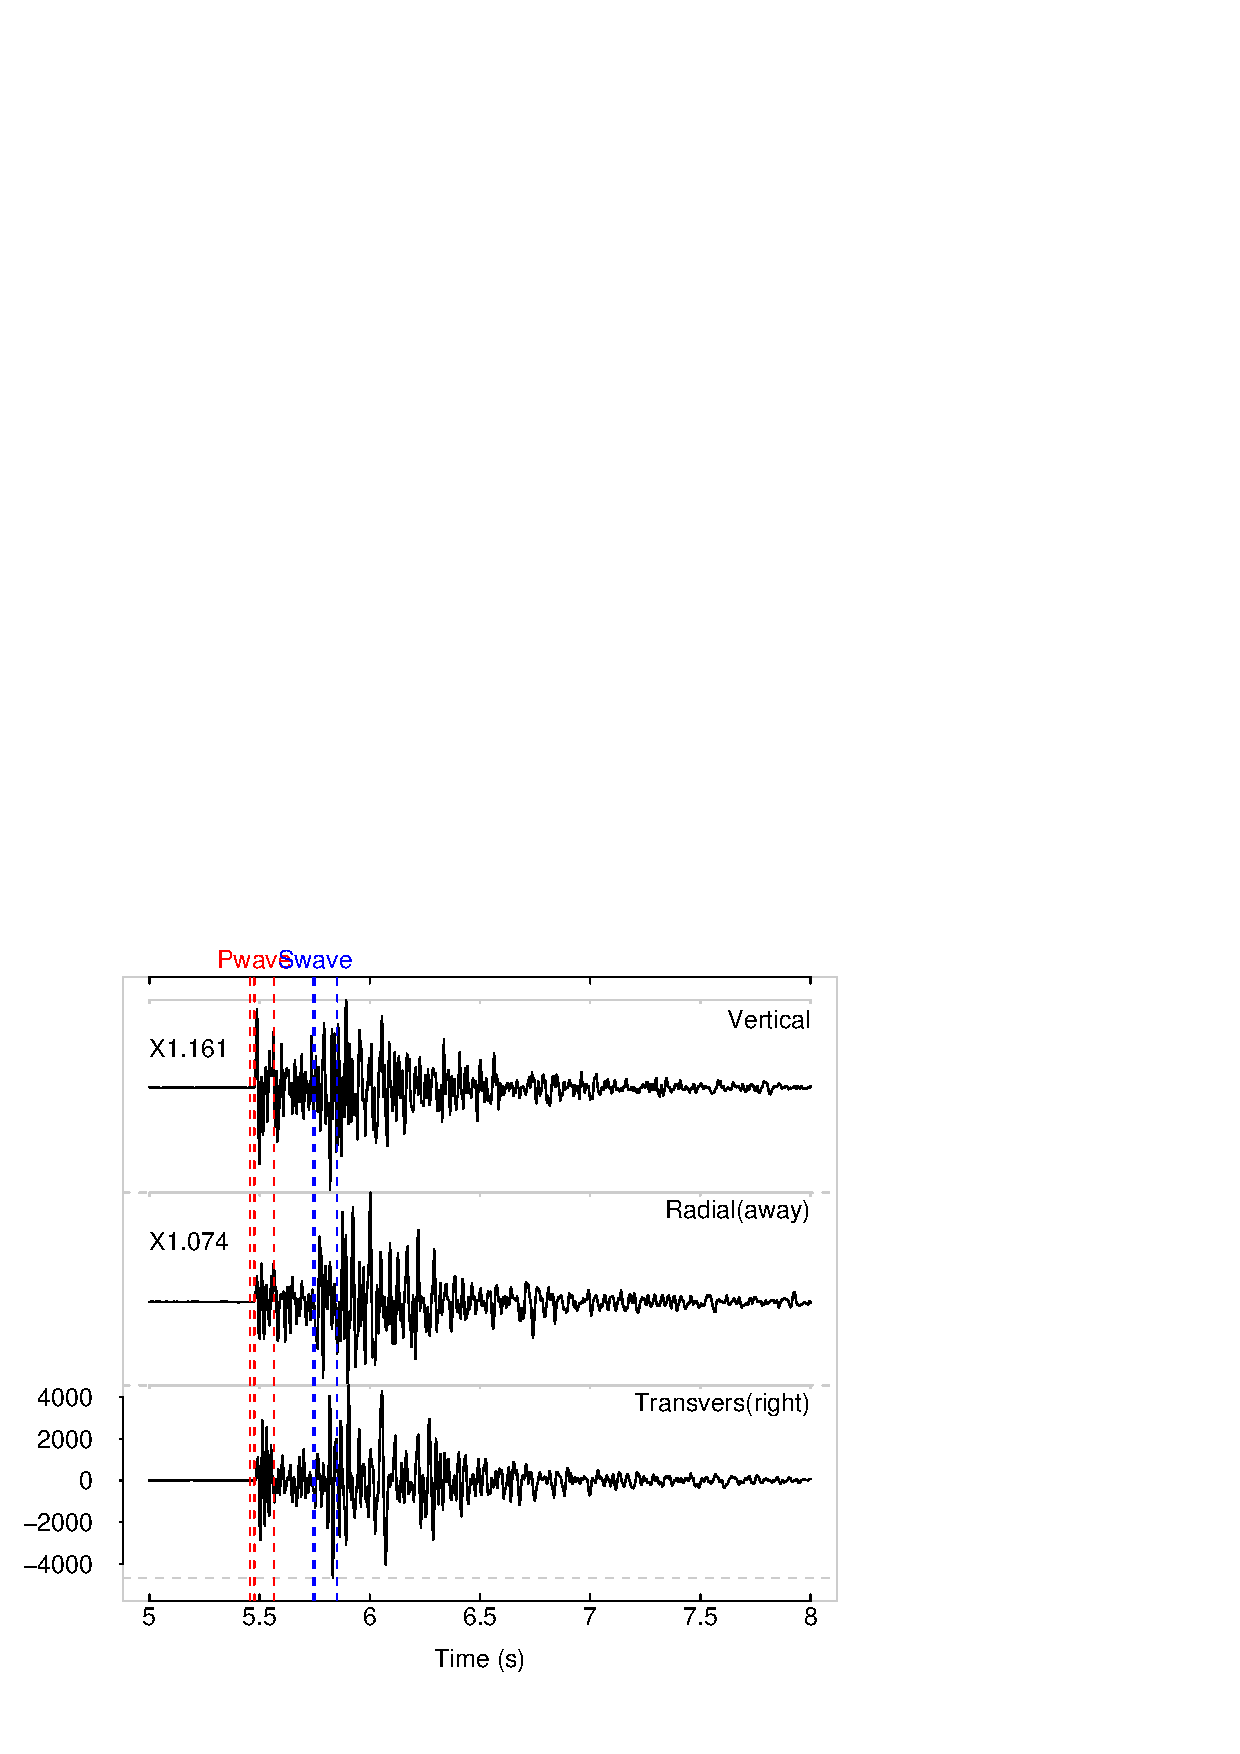
\includegraphics{hodo-010}

So we now extract that portion and apply the hodogram program
on the P-wave arrival

\begin{Schunk}
\begin{Sinput}
> rbow = rainbow(140)[1:100]
> atemp = btemp[xt > pwin[1] & xt < pwin[2], ]
> hodogram(atemp, dt = GH$dt[iwv], labs = rotlabs, STAMP = thesta, 
+     COL = rbow)
\end{Sinput}
\end{Schunk}
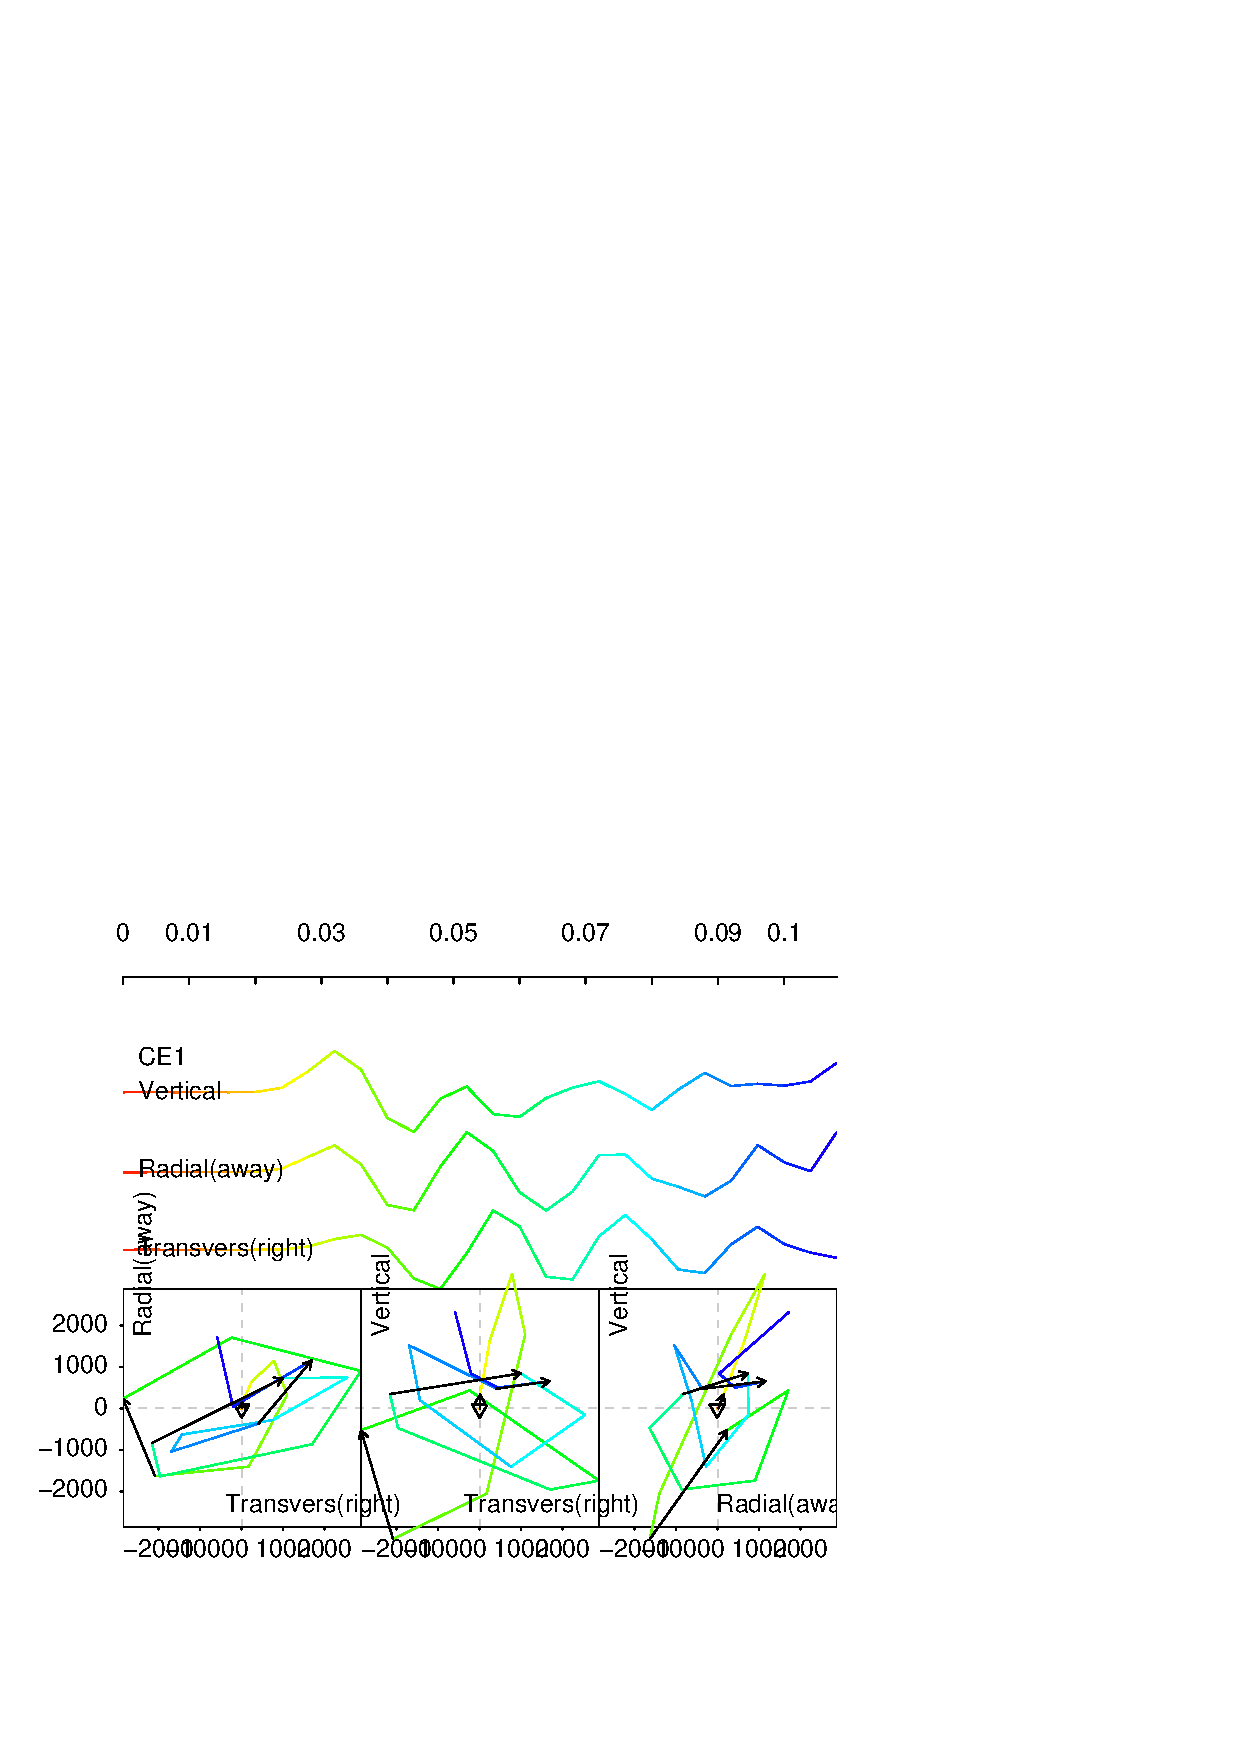
\includegraphics{hodo-011}

and on the S-wave arrival

\begin{Schunk}
\begin{Sinput}
> atemp = btemp[xt > swin[1] & xt < swin[2], ]
> hodogram(atemp, dt = GH$dt[iwv], labs = rotlabs, STAMP = thesta, 
+     COL = rbow)
\end{Sinput}
\end{Schunk}
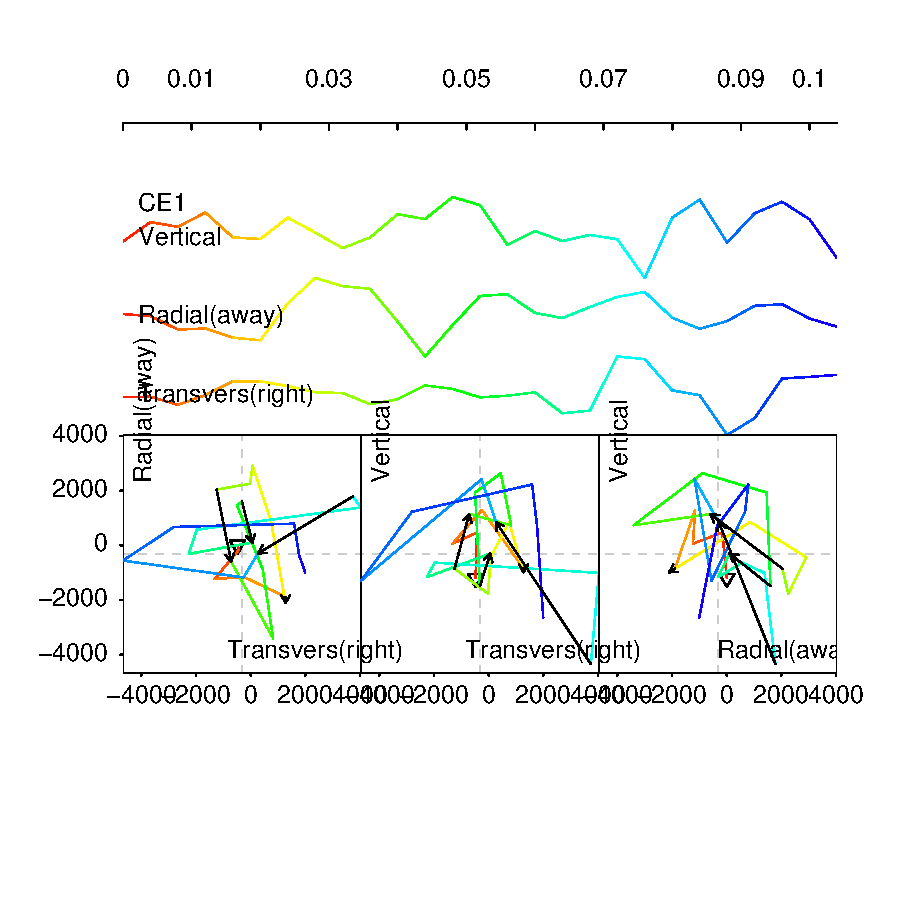
\includegraphics{hodo-012}

Clearly,  a loop
can be programed so that all the stations are examined for the 
particle motion and specific patterns will be revealed.

For example, we may wish to differentiate 
between direct arrival of body waves
and later arrivals of surface waves.
The Raleigh wave has retrograde motion int he vertical-radial 
components, so we expect to see the first motions moving 
opposite the direction of wave propagation (i.e. towards the source)
as the motion is decomposed.


Hodograms  can be used to estimate 
the arrival of a ``split shear wave'' often used to 
detect anisotropy in the geologic structures in the subsurface.
In some cases anisotropy indicates crack orientation and in the mantle 
it may refer to fluid flow as olivene crystals align
along the direction of flow.




\end{document}

